\documentclass[10pt,a4paper]{article}

\usepackage [utf8]{inputenc}
\usepackage[brazil]{babel}
\usepackage[T1]{fontenc}
%\usepackage{geometry}                % See geometry.pdf to learn the layout options. There are lots.
\usepackage{graphicx}
\usepackage{amssymb}
\usepackage{epstopdf}
\usepackage{indentfirst}
\usepackage{fancyhdr}
\usepackage{subfig}
\usepackage{wrapfig}
\usepackage{makeidx}
\usepackage[usenames]{color}
\newcommand{\todo}[1]{\textcolor{red}{\footnote{\textcolor{red}{TODO: #1}}}}
\usepackage{multirow}
\usepackage{rotating}
\usepackage{lmodern}
\usepackage{indentfirst}
\usepackage{array}
\usepackage{natbib}
%%% usado para codigo %%%
\usepackage{listings}
\lstset{
%  language = C,
  basicstyle=\footnotesize\ttfamily, 
  numbers=left,               
  numberstyle=\tiny,         
  %stepnumber=2,              
  numbersep=5pt,             
  tabsize=2,                  
  extendedchars=true,  
  breaklines=true,       
  keywordstyle=\color{blue},
%  frame=b,         
  stringstyle=\color{green}\ttfamily, 
  showspaces=false,          
  showtabs=false,             
  xleftmargin=17pt,
  framexleftmargin=17pt,
  framexrightmargin=5pt,
  framexbottommargin=4pt,
  %backgroundcolor=\color{lightgray},
  showstringspaces=false              
}
\lstloadlanguages{C}
\usepackage{caption}
\DeclareCaptionFont{white}{\color{white}}
\DeclareCaptionFont{green}{\color{green}}
\DeclareCaptionFormat{listing}{\colorbox[cmyk]{0.43, 0.35, 0.35,0.01}{\parbox{\textwidth}{\hspace{15pt}#1#2#3}}}
\captionsetup[lstlisting]{format=listing,labelfont=white,textfont=white, singlelinecheck=false, margin=0pt, font={bf,footnotesize}}


\begin{document}
%%%%%%%%%%%%%%%%%%%%%%%%%%%%%%%%%
%%%%%                                Capa                                    %%%%%
%%%%%%%%%%%%%%%%%%%%%%%%%%%%%%%%%
    \begin{titlepage}
        \begin{center} \line(5,0){350} \end{center}
        \begin{center} \huge{Laboratório 1 - Algoritmos de ordenação} \end{center}
        \begin{center} \line(5,0){350} \end{center}
        \vspace{5cm}
        \begin{center} \large{Relatório} \end{center}
        \begin{center} \large{Instituto de computação - UNICAMP} \end{center}
        \begin{center} Campinas, \today \end{center}
        \vspace{3cm}
        \begin{center} \large{Raíssa Costa Machado 097081} \end{center}
        \begin{center} \large{Matheus Ferreira Tavares Boy 103501} \end{center}


        
    \end{titlepage}
    \tableofcontents
    \clearpage
    

        
%%%%%%%%%%%%%%%%%%%%%%%%%%%%%%%%%
%%%%%                                Introdução                            %%%%%
%%%%%%%%%%%%%%%%%%%%%%%%%%%%%%%%%    
\section{Introdução}
A proposta deste laboratório é a análise prática de algoritmos de ordenação bem conhecidos: 
Insertion, Bubble, Merge, Quick e Heapsort. Implementamos os programas em C++ para cada um
desses algoritmos e testamos e avaliamos seus desempenhos, do ponto de vista dos tempos de
execução, através de um conjunto de dados contendo 50 vetores aleatórios com uma variação
de 20 a 1000 elementos com intervalos de 20. Para a análise dos piores e melhores casos
usamos 10 vetores com 100 elementos.


%%%%%%%%%%%%%%%%%%%%%%%%%%%%%%%%%
%%%%%                        Material e métodos                        %%%%%
%%%%%%%%%%%%%%%%%%%%%%%%%%%%%%%%%
\section{Modelagem}



%%%%%%%%%%%%%%%%%%%%%%%%%%%%%%%%%
%%%%%                                Estrutura                                %%%%%
%%%%%%%%%%%%%%%%%%%%%%%%%%%%%%%%%    
\section{Estrutura}


%%%%%%%%%%%%%%%%%%%%%%%%%%%%%%%%%
%%%%%                                Resultados                               %%%%%
%%%%%%%%%%%%%%%%%%%%%%%%%%%%%%%%%    
\section{Resultados}
\begin{center}
\begin{table}
\begin{tabular}{| c | c | c | c |}
\hline
Best \# & Tempo (microssegundos) & Worst \# & Tempo (microssegundos) \\ \hline 
0 & 1.2 & 0 & 94.59 \\ \hline 
1 & 1.24 & 1 & 94.71 \\ \hline 
2 & 1.21 & 2 & 94.6 \\ \hline 
3 & 1.21 & 3 & 94.5 \\ \hline 
4 & 1.22 & 4 & 94.52 \\ \hline 
5 & 1.21 & 5 & 94.49 \\ \hline 
6 & 1.22 & 6 & 94.55 \\ \hline 
7 & 1.21 & 7 & 94.53 \\ \hline 
8 & 1.21 & 8 & 94.53 \\ \hline 
9 & 1.22 & 9 & 94.49 \\ \hline 
Média & 1.215 & Média & 94.551 \\ \hline 
\end{tabular}
\caption{Tempos de execução dos piores e melhores casos do Bubble Sort}
\label{table:bubble_worst_best}
\end{table}
\end{center}


\begin{center}
\begin{table}
\begin{tabular}{| c | c | c | c |}
\hline
Best \# & Tempo (microssegundos) & Worst \# & Tempo (microssegundos) \\ \hline 
0 & 15.39 & 0 & 17.76 \\ \hline 
1 & 15.79 & 1 & 17.52 \\ \hline 
2 & 15.78 & 2 & 17.46 \\ \hline 
3 & 15.9 & 3 & 17.7 \\ \hline 
4 & 15.31 & 4 & 16.99 \\ \hline 
5 & 15.69 & 5 & 17.49 \\ \hline 
6 & 15.45 & 6 & 17.26 \\ \hline 
7 & 15.56 & 7 & 17.5 \\ \hline 
8 & 15.6 & 8 & 17.25 \\ \hline 
9 & 15.59 & 9 & 17.42 \\ \hline 
Média & 15.606 & Média & 17.435 \\ \hline 
\end{tabular}
\caption{Tempos de execução dos piores e melhores casos do Heapsort}
\label{table:heap_worst_best}
\end{table}
\end{center}


\begin{center}
\begin{table}
\begin{tabular}{| c | c | c | c |}
\hline
Best \# & Tempo (microssegundos) & Worst \# & Tempo (microssegundos) \\ \hline 
0 & 1.77 & 0 & 42.46 \\ \hline 
1 & 1.77 & 1 & 42.47 \\ \hline 
2 & 1.78 & 2 & 42.48 \\ \hline 
3 & 1.78 & 3 & 42.47 \\ \hline 
4 & 1.78 & 4 & 42.47 \\ \hline 
5 & 1.78 & 5 & 42.46 \\ \hline 
6 & 1.78 & 6 & 42.47 \\ \hline 
7 & 1.78 & 7 & 42.47 \\ \hline 
8 & 1.76 & 8 & 42.47 \\ \hline 
9 & 1.76 & 9 & 42.47 \\ \hline 
Média & 1.774 & Média & 42.469 \\ \hline 
\end{tabular}
\caption{Tempos de execução dos piores e melhores casos do Insertion Sort}
\label{table:insertion_worst_best}
\end{table}
\end{center}


\begin{center}
\begin{table}
\begin{tabular}{| c | c | c | c |}
\hline
Best \# & Tempo (microssegundos) & Worst \# & Tempo (microssegundos) \\ \hline 
0 & 13.98 & 0 & 14.78 \\ \hline 
1 & 14.01 & 1 & 14.77 \\ \hline 
2 & 14.02 & 2 & 14.78 \\ \hline 
3 & 14.03 & 3 & 14.78 \\ \hline 
4 & 14.02 & 4 & 14.78 \\ \hline 
5 & 13.97 & 5 & 14.78 \\ \hline 
6 & 13.98 & 6 & 14.76 \\ \hline 
7 & 13.96 & 7 & 14.72 \\ \hline 
8 & 14.19 & 8 & 14.78 \\ \hline 
9 & 14.15 & 9 & 14.76 \\ \hline 
Média & 14.031 & Média & 14.769 \\ \hline 
\end{tabular}
\caption{Tempos de execução dos piores e melhores casos do Merge Sort}
\label{table:merge_worst_best}
\end{table}
\end{center}


\begin{center}
\begin{table}
\begin{tabular}{| c | c | c | c |}
\hline
Best \# & Tempo (microssegundos) & Worst \# & Tempo (microssegundos) \\ \hline 
0 & 10.09 & 0 & 41.35 \\ \hline 
1 & 11.51 & 1 & 41.41 \\ \hline 
2 & 10.55 & 2 & 41.46 \\ \hline 
3 & 10.98 & 3 & 41.4 \\ \hline 
4 & 10.19 & 4 & 41.38 \\ \hline 
5 & 10.13 & 5 & 41.36 \\ \hline 
6 & 10.63 & 6 & 41.54 \\ \hline 
7 & 11.35 & 7 & 41.36 \\ \hline 
8 & 11.07 & 8 & 41.39 \\ \hline 
9 & 10.98 & 9 & 41.44 \\ \hline 
Média & 10.748 & Média & 41.409 \\ \hline 
\end{tabular}
\caption{Tempos de execução dos piores e melhores casos do Quicksort}
\label{table:quick_worst_best}
\end{table}
\end{center}


\begin{center}
\begin{table}
\begin{tabular}{| c | c | c | c | c | c |}
\hline
Random Size & Bubble & Heap & Insertion & Merge & Quick \\ \hline 
20 & 0 & 0 & 0 & 0 & 0 \\ \hline 
40 & 0.01 & 0 & 0 & 0 & 0 \\ \hline 
60 & 0.02 & 0.01 & 0.01 & 0.01 & 0 \\ \hline 
80 & 0.06 & 0.01 & 0.02 & 0.01 & 0.01 \\ \hline 
100 & 0.08 & 0.02 & 0.02 & 0.02 & 0.01 \\ \hline 
120 & 0.11 & 0.02 & 0.02 & 0.02 & 0.02 \\ \hline 
140 & 0.15 & 0.03 & 0.04 & 0.02 & 0.01 \\ \hline 
160 & 0.19 & 0.03 & 0.05 & 0.03 & 0.02 \\ \hline 
180 & 0.26 & 0.03 & 0.05 & 0.03 & 0.02 \\ \hline 
200 & 0.29 & 0.05 & 0.07 & 0.04 & 0.03 \\ \hline 
220 & 0.38 & 0.04 & 0.08 & 0.04 & 0.03 \\ \hline 
240 & 0.43 & 0.05 & 0.09 & 0.04 & 0.03 \\ \hline 
260 & 0.52 & 0.06 & 0.1 & 0.05 & 0.03 \\ \hline 
280 & 0.61 & 0.06 & 0.13 & 0.05 & 0.04 \\ \hline 
300 & 0.73 & 0.07 & 0.14 & 0.06 & 0.03 \\ \hline 
320 & 0.87 & 0.08 & 0.17 & 0.06 & 0.05 \\ \hline 
340 & 0.9 & 0.07 & 0.18 & 0.06 & 0.04 \\ \hline 
360 & 1.01 & 0.09 & 0.2 & 0.07 & 0.05 \\ \hline 
380 & 1.05 & 0.09 & 0.22 & 0.07 & 0.05 \\ \hline 
400 & 1.25 & 0.09 & 0.24 & 0.08 & 0.06 \\ \hline 
420 & 1.38 & 0.11 & 0.27 & 0.08 & 0.06 \\ \hline 
440 & 1.41 & 0.1 & 0.28 & 0.09 & 0.06 \\ \hline 
460 & 1.66 & 0.12 & 0.32 & 0.09 & 0.07 \\ \hline 
480 & 1.75 & 0.12 & 0.34 & 0.1 & 0.07 \\ \hline 
500 & 1.9 & 0.12 & 0.38 & 0.1 & 0.07 \\ \hline 
520 & 2.07 & 0.13 & 0.39 & 0.1 & 0.08 \\ \hline 
540 & 2.24 & 0.14 & 0.45 & 0.11 & 0.09 \\ \hline 
560 & 2.36 & 0.14 & 0.44 & 0.11 & 0.09 \\ \hline 
580 & 2.62 & 0.15 & 0.5 & 0.12 & 0.08 \\ \hline 
600 & 2.79 & 0.15 & 0.52 & 0.13 & 0.09 \\ \hline 
620 & 3.01 & 0.16 & 0.55 & 0.12 & 0.09 \\ \hline 
640 & 3.08 & 0.17 & 0.6 & 0.14 & 0.1 \\ \hline 
660 & 3.27 & 0.17 & 0.63 & 0.13 & 0.1 \\ \hline 
680 & 3.47 & 0.18 & 0.66 & 0.14 & 0.1 \\ \hline 
700 & 3.78 & 0.18 & 0.72 & 0.15 & 0.11 \\ \hline 
720 & 3.99 & 0.19 & 0.76 & 0.15 & 0.11 \\ \hline 
740 & 4.35 & 0.2 & 0.78 & 0.15 & 0.12 \\ \hline 
760 & 4.32 & 0.2 & 0.82 & 0.16 & 0.11 \\ \hline 
780 & 4.67 & 0.21 & 0.89 & 0.16 & 0.12 \\ \hline 
800 & 4.95 & 0.22 & 0.93 & 0.17 & 0.13 \\ \hline 
820 & 4.99 & 0.22 & 0.96 & 0.18 & 0.13 \\ \hline 
840 & 5.45 & 0.23 & 1.04 & 0.17 & 0.14 \\ \hline 
860 & 5.75 & 0.23 & 1.08 & 0.19 & 0.14 \\ \hline 
880 & 6 & 0.24 & 1.13 & 0.19 & 0.13 \\ \hline 
900 & 6.26 & 0.25 & 1.18 & 0.19 & 0.15 \\ \hline 
920 & 6.46 & 0.25 & 1.18 & 0.2 & 0.14 \\ \hline 
940 & 6.87 & 0.26 & 1.3 & 0.2 & 0.15 \\ \hline 
960 & 7.27 & 0.26 & 1.3 & 0.21 & 0.16 \\ \hline 
980 & 7.56 & 0.27 & 1.36 & 0.22 & 0.15 \\ \hline 
1000 & 7.8 & 0.27 & 1.44 & 0.22 & 0.16 \\ \hline 
\end{tabular}
\caption{Tempos de execução dos vetores aleatórios de todos os sorts}
\label{table:sorts_random}
\end{table}
\end{center}


\begin{figure}[ht]
\centering
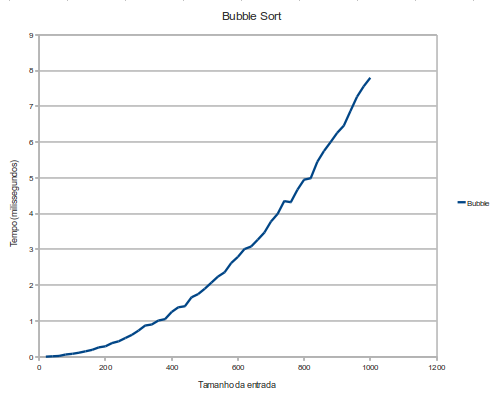
\includegraphics[width=1.2\textwidth]{bubble.png}
\caption{Gráfico de desempenho do Bubble Sort}
\label{fig:bubble}
\end{figure}


\begin{figure}[ht]
\centering
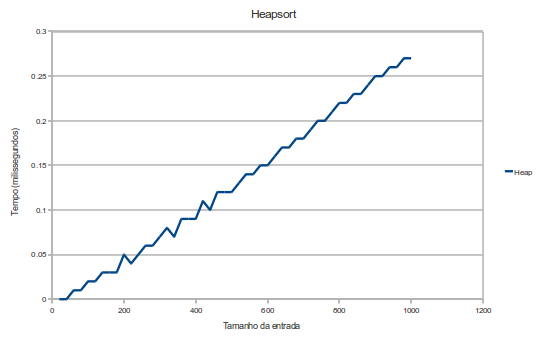
\includegraphics[width=1.2\textwidth]{heap.png}
\caption{Gráfico de desempenho do Heapsort}
\label{fig:heap}
\end{figure}


\begin{figure}[ht]
\centering
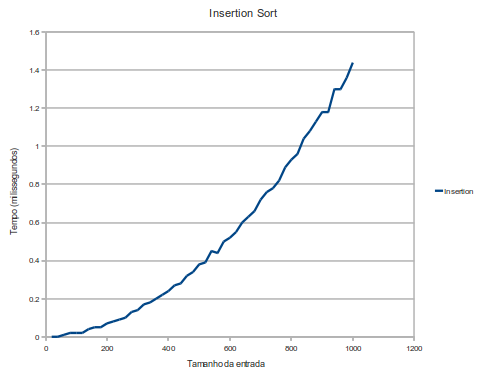
\includegraphics[width=1.2\textwidth]{insertion.png}
\caption{Gráfico de desempenho do Insertion Sort}
\label{fig:insertion}
\end{figure}


\begin{figure}[ht]
\centering
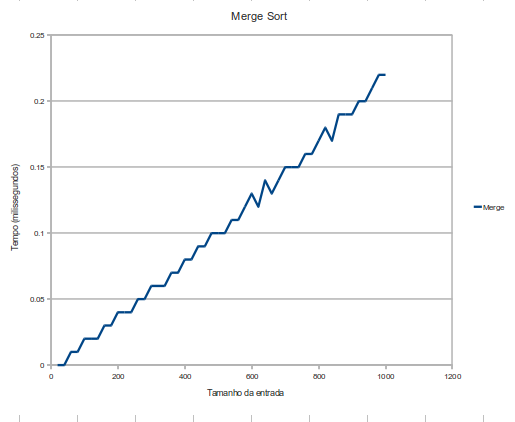
\includegraphics[width=1.2\textwidth]{merge.png}
\caption{Gráfico de desempenho do Merge Sort}
\label{fig:merge}
\end{figure}


\begin{figure}[ht]
\centering
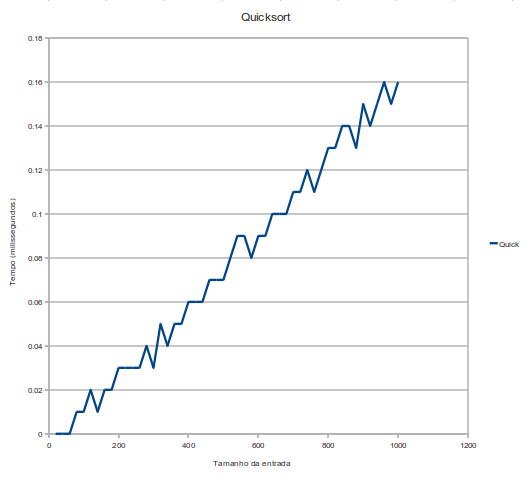
\includegraphics[width=1.2\textwidth]{quick.png}
\caption{Gráfico de desempenho do Quicksort}
\label{fig:quick}
\end{figure}


\begin{figure}[ht]
\centering
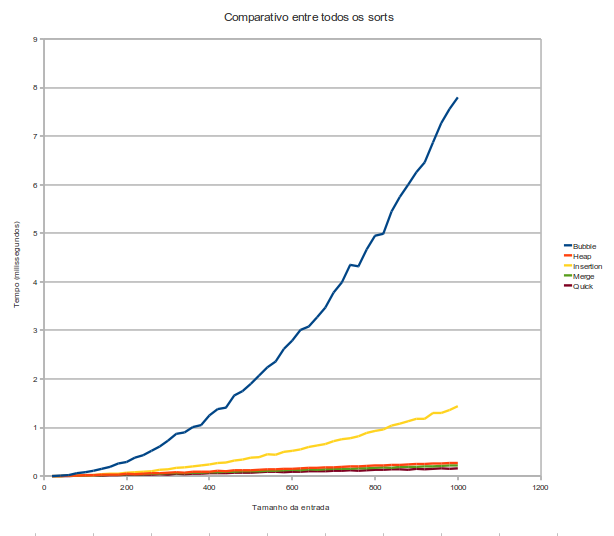
\includegraphics[width=1.2\textwidth]{all_sorts.png}
\caption{Gráfico comparativo de desempenho de todos os sorts}
\label{fig:all_sorts}
\end{figure}

%%%%%%%%%%%%%%%%%%%%%%%%%%%%%%%%%

%%%%%                               Conclusões                            %%%%%
%%%%%%%%%%%%%%%%%%%%%%%%%%%%%%%%%
\section{Conclusões}



\bibliography{Projeto.bib}
\bibliographystyle{plain}

\end{document}
